\subsection{凸性判别法}

命题 7. 设 f 是定义在区间 \(I \subset R\) 上的实值有限函数。为使 f 在 I 上是凸的，必须且只需：对 I 中满足 a \textless{} b 的每一对数 a, b，以及对每个实数 \(\mu\)，函数 \(f(x) + \mu x\) 都在点 a, b 之一处取得它在 \([a, b]\) 上的上确界。

此条件是必要的；事实上，由于 \(\mu x\) 在 \(\mathbf{R}\) 上凸，函数 \(f(x) + \mu x\) 在 I 上凸；因此可以只限于 \(\mu = 0\) 的情形。此时，对

\[
x = \lambda a + (1 - \lambda) b \quad (0 \leqslant \lambda \leqslant 1),
\]

有

\[
f (x) \leqslant \lambda f (a) + (1 - \lambda) f (b) \leqslant \operatorname{Max} (f (a), f (b)).
\]

此条件是充分的。取 \(\mu = -\frac{f(b) - f(a)}{b - a}\) 并设 \(g(x) = f(x) + \mu x\)；有 \(g(a) = g(b)\)，因此 \(g(x) \leqslant g(a)\) 对一切 \(x \in [a, b]\) 成立，并且可以立即验证这个不等式等价于把 (1) 中的 \(z\) 换成 \(a\)、\(x'\) 换成 \(b\) 所得的不等式。

命题 8. 为使实值有限函数 f 在开区间 \(I \subset R\) 上是凸的（相应地，严格凸的），必须且只需：它在 I 上连续，在此区间的某个可数子集相对于 I 的余集 B 的每一点处有导数，并且该导数在 B 上递增（相应地，严格递增）。

由命题 6 及其推论 2（I, p.~27），此条件是必要的；我们来证明它是充分的。因此假设 \(f'\) 在 B 上递增，而 \(f\) 不是凸的；于是存在（I, p.~27, 命题 5）I 的三个点 \(a, b, c\)，使得 \(a < c < b\) 且 \(\frac{f(c) - f(a)}{c - a} > \frac{f(b) - f(c)}{b - c}\)；但由中值定理（I, p.~14, 定理 1）有

\[
\frac {f (c) - f (a)}{c - a} \leqslant \sup _ {x \in \mathrm{B}, a <   x <   c} f ^ {\prime} (x) \quad \text { and } \quad \frac {f (b) - f (c)}{b - c} \geqslant \inf _ {x \in \mathrm{B}, c <   x <   b} f ^ {\prime} (x).
\]

于是有 \(\sup_{x\in \mathbf{B},a < x < c}f'(x) > \inf_{x\in \mathbf{B},c < x < b}f'(x)\)，这与 \(f'\) 在 B 上递增的假设矛盾。

若现在假设 \(f'\) 在 B 上严格递增，则 \(f\) 是凸的，且不可能在含于 I 的任何开区间上等于一个仿射线性函数，因为否则 \(f'\) 将在该区间上取常值，与假设矛盾。

推论。设 \(f\) 是区间 \(\mathbf{I} \subset \mathbf{R}\) 上的实值有限函数，连续且两次可导；为使 \(f\) 在 \(\mathbf{I}\) 上凸，必须且只需 \(f''(x) \geqslant 0\) 对一切 \(x \in \mathbf{I}\) 成立；为使 \(f\) 在 \(\mathbf{I}\) 上严格凸，必须且只需前述条件成立，并且使点 \(x \in \mathbf{I}\)（在其处 \(f''(x) > 0\)）所成的集在 \(\mathbf{I}\) 中稠密。

这由前一命题以及 I, p.~14 的推论立得。

例。*在区间 {]}0, +∞{[} 上，函数 \(x^r\)（r 为任意实数）的二阶导数等于 \(r(r - 1)x^{r - 2}\)；因此当 \(r > 1\) 或 \(r < 0\) 时它严格凸，而当 \(0 < r < 1\) 时严格凹。*

为了能表述凸性的另一个判别法，我们作如下定义：给定定义在区间 \(I \subset R\) 上的实值有限函数的图像 G 以及 I 的一个内点 a，则称过 \(M_{a} = (a, f(a))\) 的直线 D 局部在 G 上方（相应地，局部在 G 下方），若存在 a 的邻域 \(V \subset I\)，使 D 的每个含于 \(V \times R\) 的点都在 G 之上（相应地，之下）；则称 D 在点 \(M_{a}\) 处局部位于 G 上，若存在 a 的邻域 \(V \subset I\)，使 D 与 \(V \times R\) 的交等同于 G 与 \(V \times R\) 的交（换言之，若 D 同时局部在 G 上方且局部在 G 下方）。

命题 9. 设 f 是开区间 \(I \subset R\) 上的上半连续的实值有限函数。为使 f 在 I 上凸，必须且只需：对 f 的图像 G 的每个点 \(M_{x}\)，在该点处局部在 G 上方的每条直线都局部位于 G 上（在点 \(M_{x}\) 处）。

此条件是必要的：事实上，若 \(f\) 在 \(I\) 上凸，则在点 \(\mathbf{M}_a\)（属于 \(G\)，即 \(f\) 的图像）处都存在一条直线 \(\Delta\)，它支撑 \(G\)；而 \(\Delta\) 位于 \(G\) 之下，故更加局部位于 \(G\) 之下（I, p.~29）；若一条直线 \(D\) 局部在 \(G\) 之上（在点 \(\mathbf{M}_a\) 处），它就局部在 \(\Delta\) 之上，从而必与 \(\Delta\) 重合，因而局部位于 \(G\) 上（在点 \(\mathbf{M}_a\) 处）。

此条件是充分的。事实上，设它成立，并设 \(f\) 在 I 上不凸；于是存在 I 的两个点 \(a, b\)（\(a < b\)），使得有 G 的点 \(\mathbf{M}_x\) 严格位于线段 \(\mathbf{M}_a\mathbf{M}_b\) 之上（图~4）。换言之，函数 \(g(x) = f(x) - f(a) - \frac{f(b) - f(a)}{b - a} (x - a)\) 取值 \(>0\) 于 {[}a, b{]} 上；由于 \(g\) 在这个紧区间上有限且上半连续，它的上确界 \(k\)（在 {[}a, b{]} 上）有限，并且 \(>0\)，而且

\pandocbounded{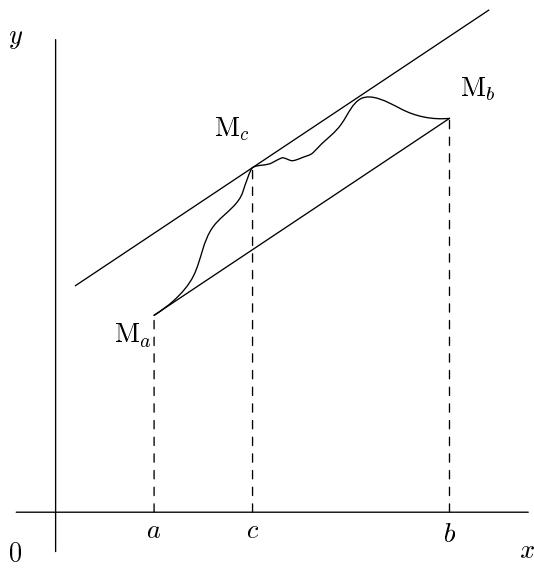
\includegraphics[keepaspectratio]{images/part001_3bcb0893.jpg}}\\
图 4

集 \(\overline{g}(k)\) 是闭的且非空（Gen.~Top., IV, p.~361, 定理 3 与命题 1）。设 c 是 \(\overline{g}(k)\) 的下确界；我们有 a \textless{} c \textless{} b，并且在点 \(M_{c}\) 处方程为 \(y = f(c) + \frac{f(b) - f(a)}{b - a}(x - c)\) 的直线 D 局部在 G 之上；但它在这一点不可能局部位于 G 上，因为对 a \textless{} x \textless{} c 有 \(g(x) < k\)，这表明 \(M_{x}\) 严格位于 D 之下。这就使我们得到矛盾，从而命题得证。

推论 1. 设 \(f\) 是定义在开区间 \(\mathbf{I} \subset \mathbf{R}\) 上且在 \(\mathbf{I}\) 上上半连续的实值有限函数；为使它在 \(\mathbf{I}\) 上凸，必须且只需：对一切 \(x \in \mathbf{I}\)，存在 \(\varepsilon > 0\)，使得关系 \(|h| \leqslant \varepsilon\) 蕴涵

\[
f (x) \leqslant \frac {1}{2} (f (x + h) + f (x - h)).
\]

我们只需证明此条件是充分的。事实上，若在 f 的图像 G 的某个点 \(M_{a}\) 处一条直线 D 局部在 G 之上，则它在该点处局部位于 G 上；因为若不然，例如，将有一个点 \(M_{a+h}\) 严格位于 D 之下，而一个点 \(M_{a-h}\) 位于 D 之下；于是线段 \(M_{a-h}M_{a+h}\) 的中点将严格位于 D 之上（图~5），而依假设，\(M_{a}\) 更加将严格位于 D 之下，这是荒谬的。

\pandocbounded{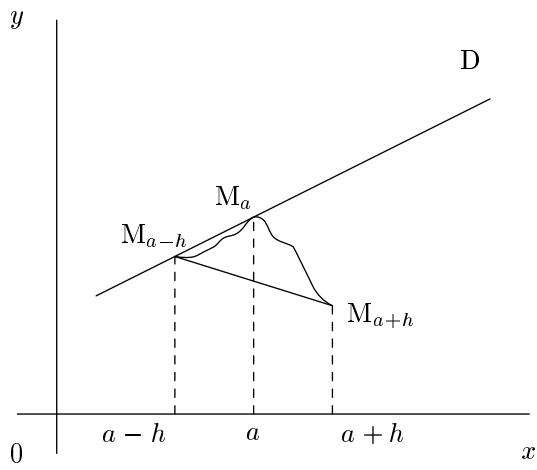
\includegraphics[keepaspectratio]{images/part001_b7dc5930.jpg}}\\
图 5

推论 2. 设 \(f\) 是定义在开区间 \(\mathrm{I} \subset \mathbf{R}\) 上的实值有限函数。若对每个点 \(x \in \mathrm{I}\) 都存在一个开区间 \(\mathrm{J}_x \subset \mathrm{I}\)，它包含 \(x\)，使 \(f\) 在 \(\mathrm{J}_x\) 上的限制在 \(\mathrm{J}_x\) 上凸，则 \(f\) 在 \(\mathrm{I}\) 上凸。

显然 \(f\) 满足命题 9 的判别法。

\setcounter{exercisegroup}{0}
\refstepcounter{exercisegroup}
